\documentclass[10pt]{article}
\usepackage[letterpaper,margin=0.5in,top=0.35in,bottom=0.35in]{geometry}
\usepackage[T1]{fontenc}
\usepackage{lmodern}
\usepackage{microtype}
\usepackage{amsmath,amssymb}
\usepackage{enumitem}
\usepackage{titlesec}
\usepackage{tikz}
\usetikzlibrary{arrows.meta,positioning,fit,calc}
\usepackage[hidelinks]{hyperref}
\usepackage{xcolor}
\usepackage{multicol}
\setlength{\columnsep}{10pt}
\setlength{\multicolsep}{2pt}
\setlength{\premulticols}{0pt}

\setlist{nosep,leftmargin=1.2em}
\titleformat{\section}{\normalsize\bfseries}{}{0pt}{}
\titlespacing*{\section}{0pt}{3pt}{1pt}
\setlength{\parindent}{0pt}
\setlength{\parskip}{2pt}
\pagestyle{empty}

\definecolor{blk}{RGB}{225,235,250}
\definecolor{lora}{RGB}{255,228,196}
\definecolor{reg}{RGB}{212,240,212}

\begin{document}
\small

\begin{center}
{\large\bfseries Do Register Artifacts Survive Parameter-Efficient Fine-Tuning?\\[1pt]
Training-Free Registers for Dense Prediction with LoRA-Adapted Vision Transformers}\\[2pt]
{\small John Roth \quad$\cdot$\quad EN.705.744 Deep Learning using Transformers, Fall 2026 \quad$\cdot$\quad Research Project Proposal}
\end{center}
\vspace{-4pt}

\section{Outline (Research Project Rubric)}
\begin{enumerate}[label=\arabic*.]
\item \textbf{Introduction \& Goals.} Register artifacts in ViTs, their cost for dense prediction, and the gap: no prior study under PEFT.
\item \textbf{Hypotheses \& Method.} Three falsifiable hypotheses; attention, LoRA and register math; block diagram (Fig.~1); ADE20K prototypes.
\item \textbf{Related Work.} Registers~[1,2], DINOv2/v3~[3,4], CLIP~[5], LoRA and vision PEFT~[6], segmentation heads~[7], maritime segmentation~[8].
\item \textbf{Application.} $3\times3$ factorial (adaptation $\times$ register condition) on three datasets, sweeps, 3 seeds, statistics, throughput.
\item \textbf{Conclusions.} The hypotheses that held, a PEFT recipe for DINOv2/CLIP dense tasks, and the reason for the study.
\end{enumerate}

\section{Problem, Candidate Solution, and Hypotheses}
\textbf{Problem.} Large pretrained ViTs (DINOv2, CLIP) develop a sparse set of high-norm ``outlier'' patch tokens in low-information regions (sky, water, walls). The model uses them as global memory, which corrupts attention and feature maps and lowers segmentation quality~[1]. Darcet et al.~[1] remove them with extra \emph{register} tokens, which requires retraining the foundation model. Jiang et al.~[2] traced the artifacts to a few ``register neurons'' in one MLP layer and removed them without training by redirecting those activations into an appended, untrained token at inference (\emph{test-time registers}). Practitioners adapt these backbones with LoRA, and no published work measures whether (a) LoRA removes the artifacts by itself, (b) test-time registers still help once LoRA is applied, or (c) the effect grows for images dominated by low-information regions.

\textbf{Candidate solution.} \emph{Register-aware PEFT}: (i) identify the register-neuron set once on the frozen backbone; (ii) insert test-time register tokens; (iii) train low-rank adapters on the attention projections and a light segmentation head, nothing else. The method adds no learned parameters over plain LoRA and needs no access to pretraining. \textbf{Research hypotheses:}
\begin{itemize}
\item \textbf{H1 (persistence).} LoRA fine-tuning leaves the outlier tokens in place: the fraction of high-norm patch tokens after LoRA stays within $\pm20\%$ of the frozen model, and vanilla LoRA scores below a backbone trained with registers on mIoU.
\item \textbf{H2 (recovery).} Test-time registers $+$ LoRA close at least 50\% of the mIoU gap between vanilla LoRA and the trained-register backbone, at equal parameter count.
\item \textbf{H3 (scaling with low-information area).} The gain grows with the fraction of homogeneous background. It peaks on maritime imagery (LaRS, where sky and water dominate) and is larger for CLIP than for DINOv2.
\end{itemize}

\section{Applied Machine Learning Method and Datasets}
\textbf{Backbones and math.} Each ViT block computes $\mathrm{Attn}(X)=\mathrm{softmax}\!\big(XW_Q W_K^{\!\top}X^{\!\top}/\sqrt{d}\big)XW_V$. LoRA~[6] freezes $W\in\mathbb{R}^{d\times k}$ and learns $W' = W + \tfrac{\alpha}{r}BA$ with $B\in\mathbb{R}^{d\times r}, A\in\mathbb{R}^{r\times k}, r\ll d$, applied to $W_Q,W_V$. We define outlier tokens as $\{i:\ \|x_i^{(\ell)}\|_2>\tau\}$ and set $\tau$ from the norm distribution of a calibration set. Following~[2], we take the register neurons $\mathcal{N}$ to be the MLP units whose activation magnitude on outlier tokens exceeds a high quantile; at layer $\ell$ we set $h_i[\mathcal{N}]\leftarrow 0$ for all patch tokens $i$ and write the removed activations to $m$ appended register tokens, which hold the global information away from the patch features. Backbones: DINOv2 ViT-S/14 and ViT-B/14 with and without trained registers (the upper bound)~[3]; CLIP ViT-B/16~[5]; DINOv3 ViT-B/16~[4] as a stretch goal.

\begin{center}
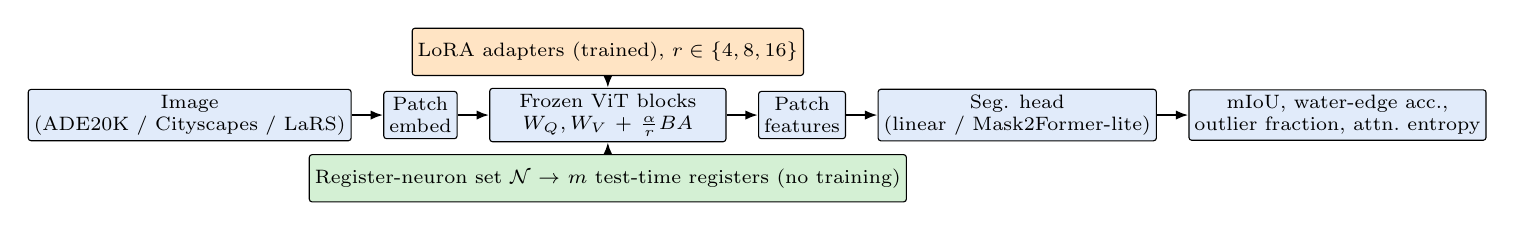
\begin{tikzpicture}[font=\scriptsize, node distance=3mm and 4mm,
  box/.style={draw,rounded corners=1pt,fill=blk,minimum height=6mm,inner sep=2pt,align=center},
  lbox/.style={box,fill=lora}, rbox/.style={box,fill=reg},
  arr/.style={-{Latex[length=1.6mm]},thick}]
\node[box] (img) {Image\\(ADE20K / Cityscapes / LaRS)};
\node[box,right=of img] (pe) {Patch\\embed};
\node[box,right=of pe,minimum width=30mm] (vit) {Frozen ViT blocks\\$W_Q,W_V$ $+$ $\tfrac{\alpha}{r}BA$};
\node[lbox,above=1.5mm of vit] (lora) {LoRA adapters (trained), $r\in\{4,8,16\}$};
\node[rbox,below=1.5mm of vit] (reg) {Register-neuron set $\mathcal{N}$ $\rightarrow$ $m$ test-time registers (no training)};
\node[box,right=of vit] (feat) {Patch\\features};
\node[box,right=of feat] (head) {Seg. head\\(linear / Mask2Former-lite)};
\node[box,right=of head] (out) {mIoU, water-edge acc.,\\outlier fraction, attn.\ entropy};
\draw[arr] (img)--(pe); \draw[arr] (pe)--(vit); \draw[arr] (vit)--(feat); \draw[arr] (feat)--(head); \draw[arr] (head)--(out);
\draw[arr] (lora)--(vit); \draw[arr] (reg)--(vit);
\end{tikzpicture}\\[-4pt]
{\scriptsize\textbf{Fig.~1.} Register-aware PEFT. Orange: the only trained backbone parameters. Green: the training-free intervention from~[2]. Ablation arms drop orange, green, or both, and we compare each against the trained-register backbone.}
\end{center}
\vspace{-6pt}

\textbf{Experimental design.} We run a factorial over adaptation $\{$frozen, LoRA, full fine-tune$\}$ $\times$ register condition $\{$none, test-time, trained$\}$ on each backbone, sweep rank $r$, target modules, number of registers $m\in\{1,4,8\}$, LoRA layer subset and learning rate, and report mean$\pm$std over 3 seeds per cell with paired tests. Heads: a linear probe, which isolates feature quality, and a light Mask2Former-style head~[7].

\textbf{Datasets and metrics.} ADE20K (150 classes, 20k train)~[9] and Cityscapes (19 classes, 2,975 train)~[10] are the standard benchmarks; LaRS~[8] ($\approx$4k per-pixel labelled maritime frames, obstacle/water/sky) is the low-information stress test for H3, scored with its water-edge accuracy and obstacle F1 as well as mIoU. Diagnostics: fraction of tokens above $\tau$, attention entropy of the CLS/register tokens, and images/s. Compute: one 24\,GB GPU; with backbones frozen, all cells fit in $\approx$8 GPU-weeks. \textbf{Timeline:} weeks 1--2 reproduce~[2] and build the outlier diagnostics; weeks 3--6 ADE20K factorial (draft due 10/19); weeks 7--10 Cityscapes and LaRS, sweeps, seeds; weeks 11--13 analysis, CLIP, writing. Venues: MaCVi workshop at WACV~2027 for the LaRS slice, then a CVPR~2027 workshop or WACV~2028 for the full study.

\section{References}
{\scriptsize\begin{multicols}{2}
\begin{enumerate}[label={[\arabic*]},leftmargin=1.6em]
\item T.~Darcet, M.~Oquab, J.~Mairal, P.~Bojanowski. Vision Transformers Need Registers. \emph{ICLR}, 2024. arXiv:2309.16588.
\item N.~Jiang, A.~Dravid, A.~Efros, T.~Darrell. Vision Transformers Don't Need Trained Registers. \emph{NeurIPS}, 2025. arXiv:2506.08010.
\item M.~Oquab et al. DINOv2: Learning Robust Visual Features without Supervision. \emph{TMLR}, 2024. arXiv:2304.07193.
\item O.~Sim\'eoni et al. DINOv3. arXiv:2508.10104, 2025.
\item A.~Radford et al. Learning Transferable Visual Models From Natural Language Supervision. \emph{ICML}, 2021.
\item E.~Hu et al. LoRA: Low-Rank Adaptation of Large Language Models. \emph{ICLR}, 2022. arXiv:2106.09685.
\item B.~Cheng et al. Masked-attention Mask Transformer for Universal Image Segmentation. \emph{CVPR}, 2022.
\item L.~\v{Z}ust, J.~Per\v{s}, M.~Kristan. LaRS: A Diverse Panoptic Maritime Obstacle Detection Dataset and Benchmark. \emph{ICCV}, 2023.
\item B.~Zhou et al. Scene Parsing through ADE20K Dataset. \emph{CVPR}, 2017.
\item M.~Cordts et al. The Cityscapes Dataset for Semantic Urban Scene Understanding. \emph{CVPR}, 2016.
\end{enumerate}\end{multicols}}

\end{document}
